% Introduction
%
%	Motivation
%	State of the Research
%	Goals and Outline

% to have the full description again
\glsreset{FFT} 
\glsreset{GPU}
\glsreset{ADT}
\glsreset{LHC}
\glsreset{tune}

\chapter{Introduction}

The \gls{LHC} is a particle collider situated between the French and Swiss boarder near Geneva. It accelerate two beams of proton to an energy of 7 Tev per beam and collide them in an interaction point, where experiment are located. The goal of the \gls{LHC} is to access and discover new physic beyond standard model.

To increase the life time of the beam in the machine and therefor increase the physic time, better parameter acquisition and correction is needed. One of the key parameter of an accelerator is the \gls{tune}.

\section{Description of the betatron tune}

In a particle accelerator, the charged particles circulate around the ring and oscillate due to the magnets and the accelerating structures. The accelerating structures in the \gls{LHC} supra-conducting \glspl{cavity} apply a strong electrical field that oscillates at the \gls{rffreq} keeping the particles longitudinally focused, in the direction of flight forming a packet, called a \gls{bunch}.

The particles inside a bunch oscillate longitudinally within the so called bucket, the area limited by the largest possible closed trajectory in time-energy phase space and transversally in the vertical and horizontal plane. The longitudinal oscillations are damped by the beam control system. Transversal oscillations are damped by a separate system~: the \gls{ADT}\cite{Zhabitsky:1141925,Benews11}.

One of the key parameters of the accelerator is the betatron tune defined by the arrangement and strength of defocussing and focusing quadrupoles around the ring. The betatron tune, $Q$, in the horizontal (respectively vertical) plane is defined as the number of oscillations per revolution within the griding magnetic fields around the accelerator.

% Literacy survey
\section{Tune measurement in the LHC}

In order to measure the betatron tune in an accelerator, we use \glspl{BPM}. Which are able to measure the position of the beam in the vacuum chamber. (TODO description of the working)

Presently the \gls{BI} group is using a \gls{BBQ} \cite{Boccardi:1156349} system to acquire the tune over a certain number of machine turns (256 to 128'000). This system can work as a passive instrument without further excitation of the beam or as an on demand system by exciting (increase oscillation amplitude) a limited number of \glspl{bunch} in the beam with the \gls{MKQA}. The \Gls{ADT} has also been used for tune measurement excitation\cite{HofleEvian10}. The \gls{BBQ} system makes an average over a certain number of bunches in the machine and is not able to see individual bunches.

In normal operation, when the \gls{ADT} is active, it is difficult to have a good picture of the excited bunches and make a precise tune measurement~: the oscillations created by the \gls{MKQA} are rapidly damped by the \gls{ADT}. There have been studies to disable the \gls{ADT} for a certain number of bunches in order to get a better tune measurement\cite{HofleEvian11}, but this may not be sufficient.

% The source of Ideas
\section{Proposed system}

The \gls{ADT} also has \glspl{BPM} assigned to it with electronics installed that permit a bunch-by-bunch measurement at the $\mu$m level\cite{BphMeas07}. This could allow a much more precise measurement on single bunches. Due to the high amount of data to be processed (estimated to 640 mega-bytes per second for each \gls{BPM}) dedicated hardware is needed to compute the correct tune using all information available\cite{HofleChamonix12}.

As the time measurements are used in the so called ``tune feedback'' to directly feed back to the focusing and defocussing magnets, a high rate of measurements is needed with tight constraints on the delays. In order to be able to apply the correction to magnets, the \gls{tune} has to be measured at a rate between 5 and 10 Hz, once every 100 to 200 ms.

During the 2012 normal operation of the \gls{LHC}, data has be acquired using the \gls{ADT} acquisition system and different data processing techniques have been tested to asses the modification that will be needed in order to make a reliable \gls{tune} measurement at a reasonable rate\cite{HofleChamonix12}.

The current \gls{VME} implementation has some serious issues, since the bus has a quite low data rate of around 40 megabits per seconds. The data need to either be processed on the acquisition board or to be off-loaded to another computer using the serial link available on the board\cite{Baudrenghien:1124094}.

\subsection{DSP on VME board}

\Glspl{DSP} are dedicated microprocessors that can perform digital signal processing such as computing \glspl{FFT} at a high rate. These are already used in the machine at different places to provide high speed feedback loops. we may ask the question~: is it fast enough to compute all the \glspl{FFT} needed? \glspl{DSP} are two orders of magnitude slower than \glspl{GPU} for delivering floating-point operation per seconds. We also would have to develop a completely new system in order to be able to use them, since in fact we don't have \glspl{DSP} in the present \gls{ADT}. The cost of development and the complexity of the deployment would have to be studied for such a solution.

\subsection{FPGA pre-processing on VME board}

Like in the approach using \gls{DSP} on VME boards, the question of computing power is an important one. The current \gls{ADT} system only features \glspl{FPGA} on the hardware, complemented by the general purpose \gls{CPU} in the \gls{VME} crate.  

The biggest issue for \gls{FPGA} computing is the fact that you need something like a \~100 mega-bytes of memory to store the temporary values for computation of only one beam plane. The \glspl{FFT} are difficult to pipeline because you have to iterate the algorithm a certain number of time ($\log_{2} N$ times for a radix 2).

\subsection{GPU off-board computing}

This solution can be integrated easily within the present setup. The present acquisition cards already have a digital output and could be used to transfer the data to another crate for the computations. The \glspl{GPU} are inexpensive (compared to the price of developing a new \gls{VME} card) and easily scalable. 

The \gls{GPU} should have sufficient computing power to be able to make the \glspl{FFT}. The \gls{FFT} computation are made in floating point. Another interesting aspect of this solution is the ability to test it with a \gls{CPU} using the same code.

\section{GPU Solution constraints}

Show how to implement a GPU based system that can deliver a tune value for each beam and plane at a rate that allows the system to be responsive enough for a tune correction to be applied automatically. 

   \subsection{Algorithm}

   To obtain the tune frequency from the tune position of the \glspl{bunch}, we have to calculate the FFT to move from time to frequency domain. Then we need to identify the tune in the transformation.

   \subsection{Hardware}

   \begin{figure}[H]
	\caption{ADT acquisition hardware}
	\centering
	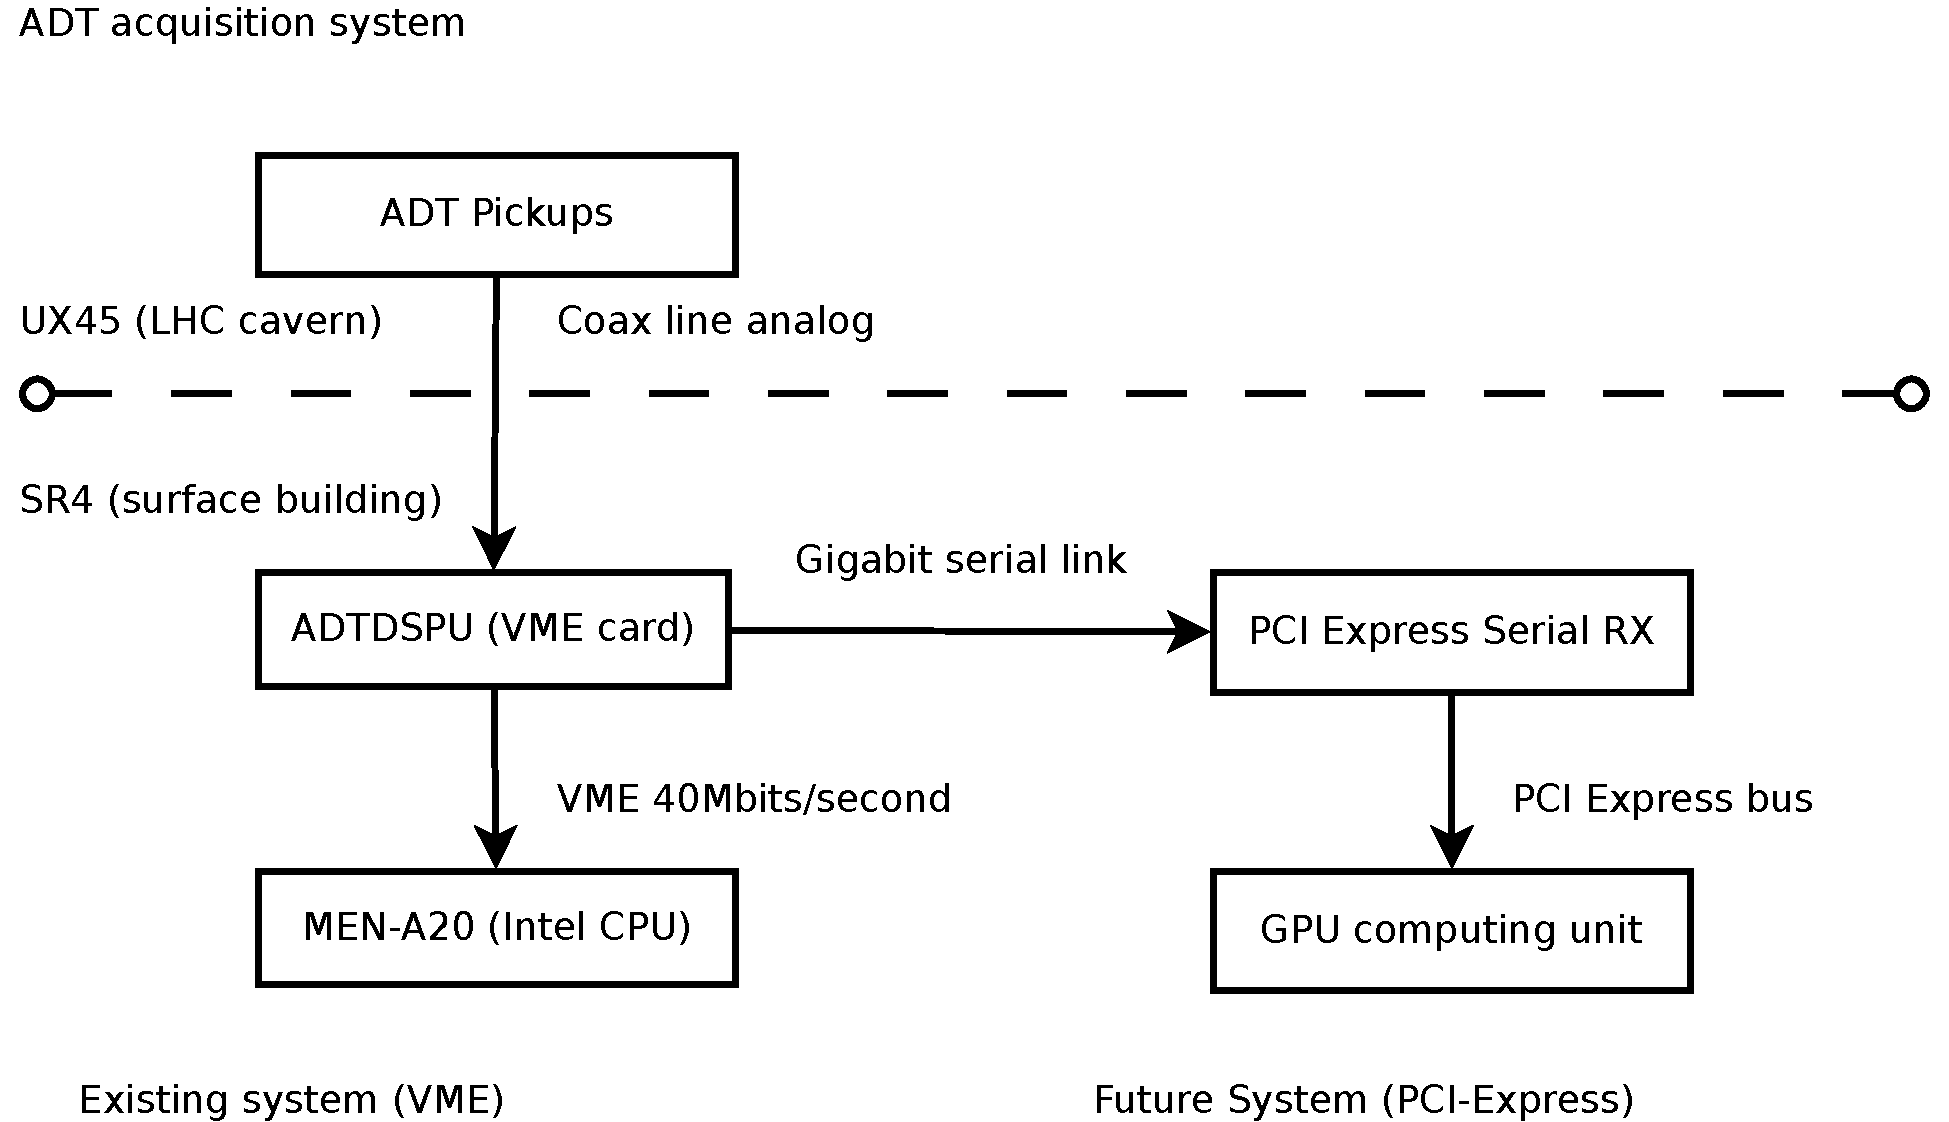
\includegraphics[scale=0.3]{acquisition.pdf}
	\end{figure}

   Per bunch position measurement has to be available to the system for each beam and each plane. This should be provided by the \gls{ADTDSPU} card and has to be transfered through a serial link to the CPU/GPU crate for computation.

   We need a card in the CPU/GPU crate to de-serialize the data and transfer them to the GPU memory. It may be possible to copy from the acquisition card directly to the GPU memory.

   And finally we of course require fast enough GPU to process the data. The number and the type of cards should be carefully looked at. The possibility for expansion should be kept in mind as the possibility to implement other algorithms.
   
   \subsection{Timings}

   According to the \gls{BI} group we have to provide the tune measurement at a rate of between 5 Hz and 10 Hz delay. This mean that the transfer and the computation has to be made in less than 200 ms.

   At a higher frequency because of the acquisition frequency (11 kHz) the precision may be insufficient (Nyquist$-$Shannon sampling theorem).